\documentclass[conference]{IEEEtran}
\usepackage{lettrine}
\usepackage{placeins}
\usepackage{tabularx}
\usepackage{graphicx}
\usepackage[strings]{underscore}
\usepackage[normalem]{ulem}
\usepackage{float}
\usepackage{caption}
\useunder{\uline}{\ul}{}

\DeclareUnicodeCharacter{200A}{} 

\begin{document}

    \title{Deep Neural Network with Raspberry Pi}
    \author{
        \IEEEauthorblockN{Lauro Cabral}
        \IEEEauthorblockA{
            Department of Engineering\\ 
            California State University of Long Beach\\
            Lauro.Cabral@student.csulb.edu
        }
        \and
        \IEEEauthorblockN{Sotheanith Sok}
        \IEEEauthorblockA{
            Department of Engineering\\ 
            California State University of Long Beach\\
            Sotheanith.Sok@student.csulb.edu
        }
    }
    \date{October 17 2020}
    \maketitle

    \begin{abstract}
        As the price of GPUs continues to increase, it has become increasingly difficult for average consumers to obtain the necessary hardware for experimenting with neural networks at home. Fortunately, it is possible to train a neural network through other means and this paper aims to explore the possibility of using distributed systems to do so. By combining Dask, a highly efficient library for parallel computing, and Raspberry Pi, a relatively cheap single-board computer, it is possible to create a cluster with a high degree of scalability that is efficient at solving deep learning problems. Additionally, such a setup is also beneficial in terms of hardware flexibility as any Raspberry Pi can be replaced with other hardware including an Intel-based system and an AMD-based system without sacrificing the performance. Lastly, by using Dask as the backend library, the current setup can be adapted to work with many popular deep learning libraries including Tensorflow and Scikit-Learn with minimal code modification while maintaining a similar result.
        \end{abstract}

    \section{Introduction}
        \IEEEPARstart{I}n the last few years, the field of deep learning has seen tremendous advancement that enables the creation of many life-changing technologies including autonomous driving, self-taught AI, and pattern recognition. This progress is only possible due to the availability of high-performance GPUs which excel at solving multiple floating pointing problems concurrently.
        According to PassMark Software, a crowd-sourced GPU benchmark database, the current flagship GPU is approximately 25000 times faster than the flagship GPU from 20 years ago \cite{passmark_software}. 

        \begin{figure}[!htb]
            \centering
            \captionsetup{justification=centering}
            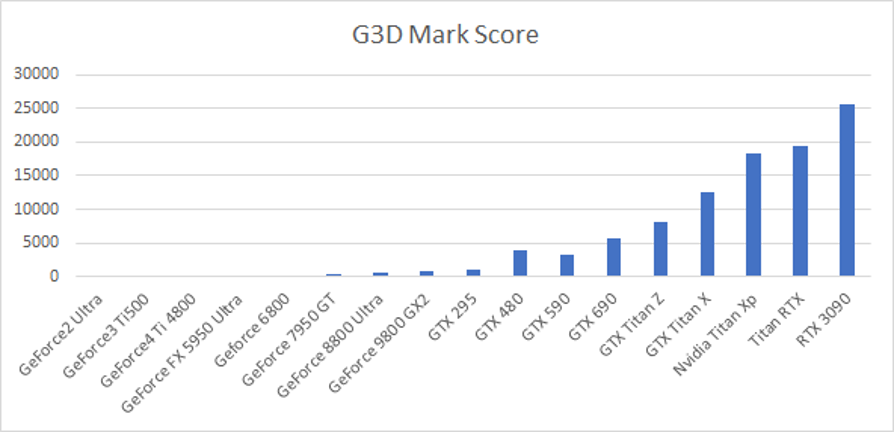
\includegraphics[width=\linewidth]{GPU_Improvment.png}
            \caption{Generational Improvement of Nvidia Flagship GPUs}  
        \end{figure}
        
        Unfortunately, the increasing interest in the field of deep learning has driven up the demand and the price of high-performance flagship GPUs exponentially. Today, a high-end flagship GPU is approximately 4 times as expensive as a flagship GPU from 20 years ago \cite{passmark_software} and these price increases make it difficult for average consumers to obtain the necessary hardware for experimenting with the deep neural network at home. As such, this paper is intended to examine the possibility of utilizing a cluster of Raspberry Pis to solve deep learning problems. Additionally, the history of deep learning which includes its initial hurdles, its rise, and the current obstacles along with the basics of deep learning including the forward-propagation, the backpropagation, and techniques for parallelizing deep learning problems will also be discussed. Furthermore, the implementation of the Raspberry Pi cluster including its setup, performances, advantages, and limitations will be explained. Finally, the last section of the paper will contain recommendations and discussions of future works.

        \begin{figure}[!htb]
            \centering
            \captionsetup{justification=centering}
            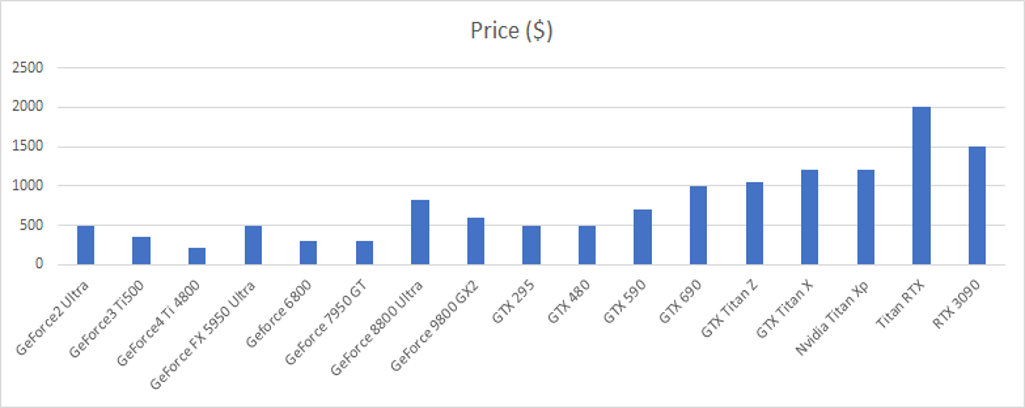
\includegraphics[width=\linewidth]{GPU_Price.png}
            \caption{MSRP of Nvidia Flagship GPUs}  
        \end{figure}

    
    \section{History of Deep Learning}
        Since its initial conception in 1967 by Alexey Ivakhnenko, the two major hurdles of applying deep neural networks in solving real-life problems are hardware limitation and data limitation. To start with, a majority of hardware designed at that time was focused on a single-core performance because that was what a majority of applications required \cite{inproceedings}. Thus, there was not an incentive for developing hardware that has more than a single core. Unfortunately, this single core focus hardware is terrible at solving neural network problems because it has to solve each node in a layer sequentially before it can proceed to the next layer. Secondly, since the internet was not widespread at the time, any dataset that needed to train a neural network has to be collected manually \cite{pew_research_center} and such a process is prohibitively expensive as good datasets are hard to come by. These hardware restrictions and data constraints stifled any advancement in the field for many years to come.

        \begin{figure}[!htb]
            \centering
            \captionsetup{justification=centering}
            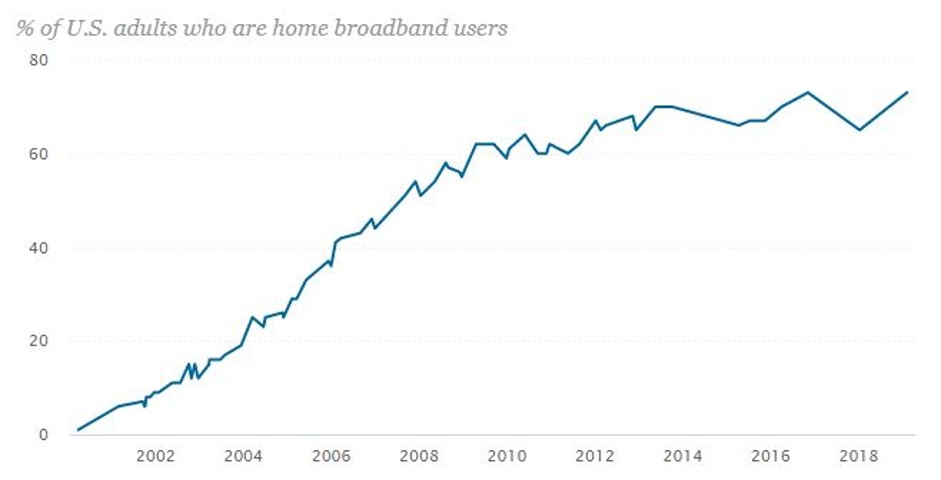
\includegraphics[width=\linewidth]{USBroadband.png}
            \caption{Percent of U.S. adult who are home broadband users}  
        \end{figure}

        The rise of deep learning in the last few years is the result of the widespread availability of high-performance GPUs which were primarily designed for rendering complex and dynamic scenes in real-time \cite{nickolls_dally_2010}. Interestingly, rendering dynamic scenes and training neural networks require similar forms of hardware solutions which compose of many fast floating-point calculating cores. With the rise of the internet and the way people interact with it, it has become easier and cheaper than ever to collect a massive amount of datasets \cite{deng_dong_socher_li_li_fei-fei_2009}. These two factors fuel the deep learning revolution that occurring today and neural networks are now adapted to solve problems that were considered too complicated for a computer to solve.
        
        However, as the field of deep learning continues to make massive progress, new problems are rearing their heads and threatening the potential growth of the field. Today, the general consensus on how to improve a neural network is to make it wider and deeper which, in theory, should increase the network representative power. However, as the network gets more complicated, it also requires more datasets to train properly. As a result, the current state of the art neural networks is composed of hundreds of nodes and layers and require millions of datasets to train. This exponential increase in the volume of information means that neural networks of today have outgrown the information capacity of most modern hardware. To simply put it, neural networks are getting too large for a majority of GPUs to represent and its training datasets are too big for most computers to store in their memories \cite{ben-nun_hoefler_2019}. To address the hardware restriction described above, many researchers have turned to the distributed system as a possible solution. The common setup for such a system is a cluster of one to many computers where each computer has as many GPUs as the computer's PCI-E bandwidth allows which is around two to four.  Even though such a setup has shown promising results, its cost is undoubtedly high and as such, it is a great barrier of entry for most consumers which, ultimately, could harm the future growth of deep learning as a field.
        
    \section{Deep Learning Basic}
        At its fundamental idea, a deep neural network is a universal approximator which means that it can estimate any function by observing said function's inputs and outputs. A deep neural network can achieve this due to its structure of multiple layers of neurons, weights, and biases \cite{hornik_1991}. For a neural network to approximate any function, it first needs to go through a training process where its weights need to be adjusted based on how accurate its predicted outputs are compared to the true outputs. This training process includes two distinct phases: forward-propagation and backpropagation. 

        \begin{figure}[!htb]
            \centering
            \captionsetup{justification=centering}
            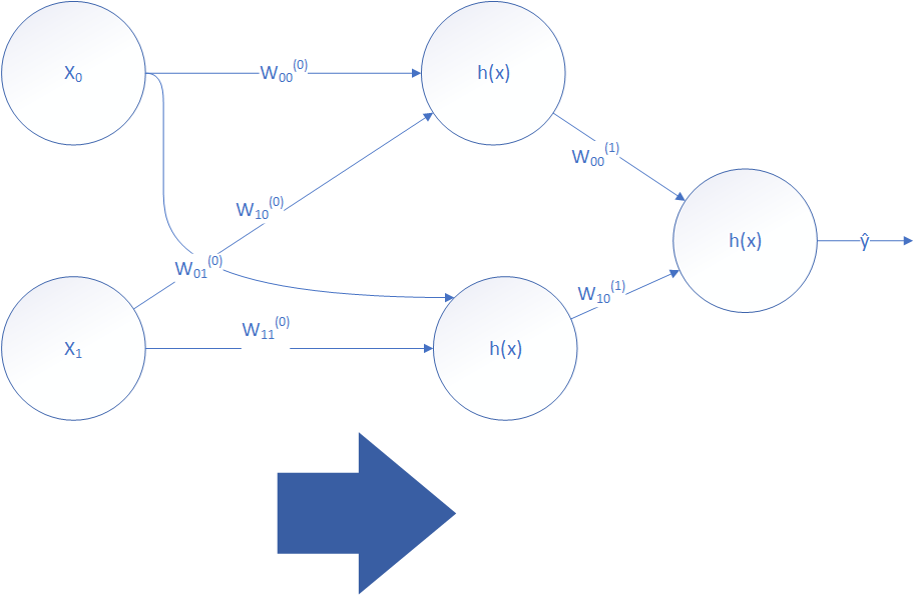
\includegraphics[width=\linewidth]{ForwardProp.png}
            \caption{Forward-Propagation: Inputs flow from left to right}  
        \end{figure}

        To start with, the main purpose of the forward-propagation phase is to see what kind of outputs are produced by a network given some inputs. This process starts by feeding inputs into the first layer and forwards outputs from such layers to the next layers. Inside each layer, neurons are responsible for taking outputs of previous layer neurons and multiplying them with their respective connection weights. Then, the neuron accumulates the resulting values and passes the sum into some kind of activation function to produce the output for this neuron. It is worth noting that the activation function is necessary for deep neural networks in order to introduce some form of nonlinearity which enables the network to approximate nonlinear function \cite{luhaniwal_2020}. This process of passing outputs from one layer to the next is repeated until the final output is achieved.

        \begin{figure}[!htb]
            \centering
            \captionsetup{justification=centering}
            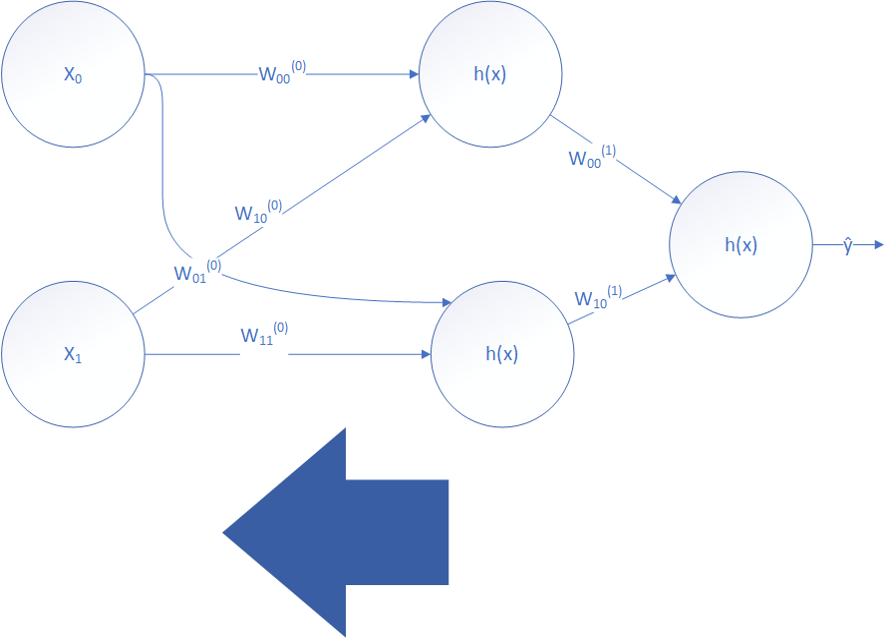
\includegraphics[width=\linewidth]{BackwardProp.png}
            \caption{Backpropagation: Loss flows from right to left}  
        \end{figure}

        Initially, the predicted outputs produced by the network will be wildly inaccurate when compared to the expected outputs due to its weights being randomly generated. However, those inaccuracies or errors do offer a hint on how to adjust the network’s weights to improve its performance. The main objective of the backpropagation phase is to adjust the network’s weights such that its errors are minimized and it accomplishes this by using the gradient descent algorithm. First off, predicted outputs and expected outputs are compared to produce an error value called loss. Then, the loss value is propagated backward throughout the network where, at each layer, the gradient, which is the amount in which each weight contributed to the loss value, gets calculated. Finally, each weight gets adjusted with their respective gradients and the entire process repeats itself until the loss is minimized \cite{kostadinov_2019}.

        At first glance, one would assume that the process of forward-propagation and backpropagation are repeated for each pair of input and output and that would produce a well-trained network but this is not necessarily the case \cite{ruder2017overview}. The major problem that arises from adjusting weights for every dataset is the instability that would be introduced into the network and thus, increases the chance of the network to converge on a suboptimal solution. Due to this uncertainty, it is recommended to train a network in batches of datasets which entails performing forward-propagation steps for multiple datasets, average their losses, and use the average loss to perform backpropagation. 

    \section{Parallelization of Deep Learning}
        The consensus on how to deal with neural networks require more resources than what modern hardware can provide is through the use of distributed systems. However, in order for neural networks to be able to run on a distributed system, its structure needs to be changed and there are two ways of doing so: data parallelization and model parallelization.

        \begin{figure}[!htb]
            \centering
            \captionsetup{justification=centering}
            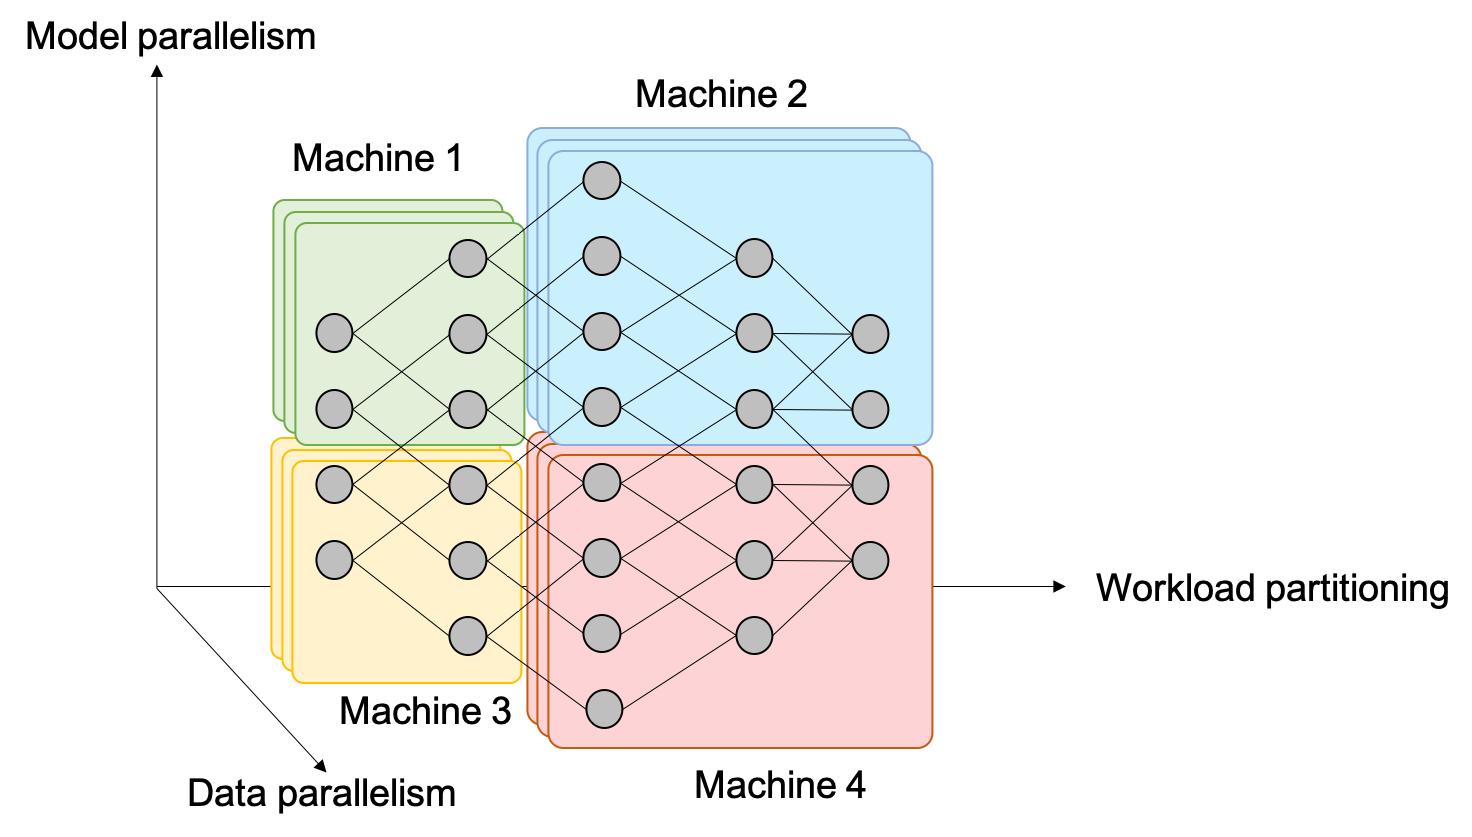
\includegraphics[width=\linewidth]{Parallelism.png}
            \caption{Model Parallelism vs Data Parallelism \cite{ekanayake}}  
        \end{figure}

        To begin with, as network networks become more complicated, its hardware requirement also increases. Thus, the goal of model parallelization is to address the scenario where networks are too deep or too wide to be represented in a single GPU. This methodology calls for the slicing of networks into smaller groups of layers where each layer chunk can be loaded onto a separate GPU. Afterward, the training process occurs similarly to how a network gets trained on a single GPU but instead of passing values from one layer to another, values are passed from one GPU to another GPU \cite{ben-nun_hoefler_2019}.

        Unfortunately, as neural network complexity increases, the amount of datasets required to train such a network also increases to the point where it exceeds the storing capacity of most computers. As such, data parallelization aims to address this issue by splitting datasets into small chunks and distributing them onto multiple nodes. Next, each node processes its chunk of datasets independently and forward the average loss either to a central node for a centralized architecture or to the next node for a map-reduce architecture. Finally, the accumulated loss gets averaged out based on the number of nodes in the cluster and the averaged loss propagates back onto all nodes where their weights get adjusted by their respective gradients \cite{ben-nun_hoefler_2019}.

    \section{Setup}
        In this experiment, software and hardware have been chosen such that it maximizes performance, flexibility, and usability while minimizes cost. 
        
        \begin{figure}[!htb]
            \centering
            \captionsetup{justification=centering}
            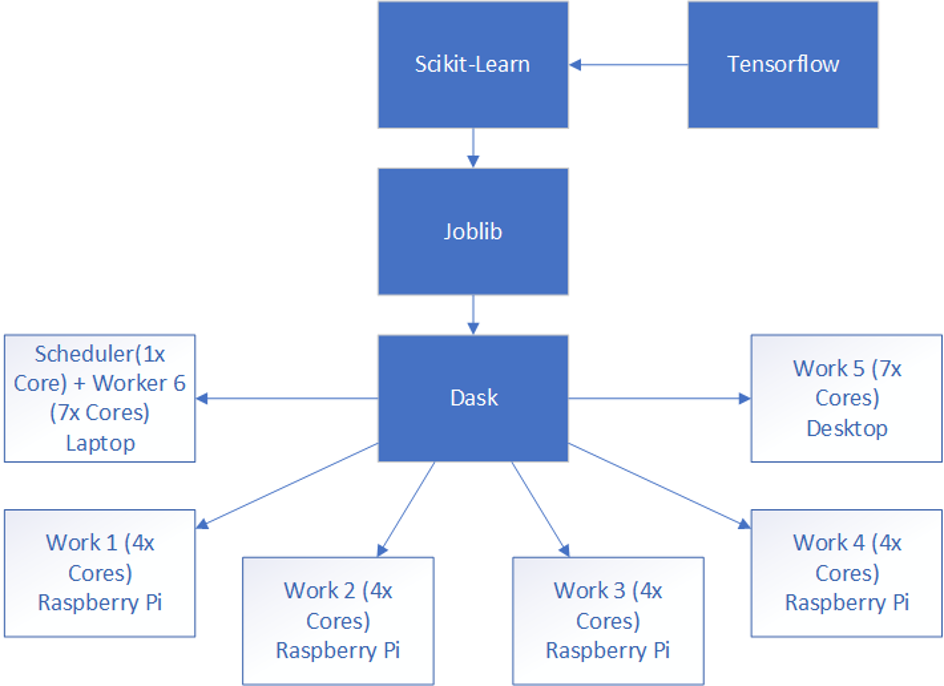
\includegraphics[width=\linewidth]{Stack.png}
            \caption{Hardware and Software stack}  
        \end{figure}
            
        The hardware stack consists of 4 Raspberry Pis, a laptop, a desktop, and a consumer-grade router and all nodes are connected to the router with ethernet cables in order to limit the inter-node communication latency. To start with, the desktop and the laptop contribute 7 computing cores each and 9 and 13 gigabytes of memories respectively to the cluster while the desktop also provides a single core as the scheduler. Then, there are 4 Raspberry Pis which contribute 4 computing cores and 2 gigabytes of memories each to the cluster. In total, the cluster will have up to 30 computing cores and 30 gigabytes of memories.

        \begin{table*}[!htbp]
            \centering%
            \begin{tabular}{|p{2cm}|p{2cm}|p{2cm}|p{4cm}|p{4.5cm}|p{2cm}|}
            \hline
            \centering{ \ul \textbf{Hardware}}        & \centering{\ul \textbf{Computing Cores}} & \centering{\ul \textbf{Memory (GB)}} & \centering{\ul \textbf{Ideal Execution Time (seconds)}} & \centering{\ul \textbf{Measured Execution Time (seconds)}} & {\centering{\ul \textbf{Scalability}}} \\ \hline
            1 x Raspberry Pi                          & 4                                        & 2                                    & 901                                                     & 901                                                        & 1                                      \\ \hline
            1 x Raspberry Pi, 1 x Desktop             & 11                                       & 11.21                                & 327.6363636                                             & 237                                                        & 1.382431914                            \\ \hline
            2 x Raspberry Pi, 1 x Desktop             & 15                                       & 13.14                                & 240.2666667                                             & 181                                                        & 1.327440147                            \\ \hline
            3 x Raspberry Pi, 1 x Desktop             & 19                                       & 15.08                                & 189.6842105                                             & 152                                                        & 1.247922438                            \\ \hline
            4 x Raspberry Pi, 1 x Desktop             & 23                                       & 17.02                                & 156.6956522                                             & 134                                                        & 1.169370539                            \\ \hline
            4 x Raspberry Pi, 1 x Desktop, 1 x Laptop & 30                                       & 29.57                                & 120.1333333                                             & 124                                                        & 0.968817204                            \\ \hline
            \end{tabular}
            \caption{Ideal execution time vs actual execution time for clusters training Random Forest Classifier}
        \end{table*}
        
        For the software stack, the choice of libraries is determined by the programming language and the availability and the maturity of libraries for implementing deep learning problems. The language of choice for this software stack is Python because of its simplicity and the availability of many popular and mature libraries such as NumPy, Scikit-Learn, Panda, and Tensorflow. These libraries are important because they streamline the implementation of many modern deep learning models. Since Python is the language of choice, the obvious pick of distributed system management library is Dask, a popular open-source library for parallel computing written purely in Python. In addition, Dask also provides native support for running a deep learning model on a cluster with the help of Dask-ML and JobLib libraries which act as middlewares between Dask and Scikit-Learn. 

    \section{Results}   
        For any experiment, it is important to establish a baseline result such that any subsequent results can be measured relative to it. After examining all the available models provided by Scikit-Learn, the Random Forest Classifier is picked as the test model because it achieves the best performance during the test run with the maximum size cluster. Thus, a single Raspberry Pi is used to train the classifier and its performance will act as the baseline result. It takes the Raspberry Pi 901 seconds to complete the execution and this result is expected since the 4 computing cores of Raspberry Pi are relatively slow compares to modern computing cores. 
            
        Next, by combining the computing cores of a Raspberry Pi and the desktop, the cluster's computing cores increases to 11 and it takes this cluster 237 seconds to train the classifier which translates to 138\% cores scaling efficiency. The abnormally high scaling efficiency is a strong indication that the scheduler is able to take full advantage of hardware heterogeneity and allocate more works to faster computing cores of the desktop. Increasing computing cores by adding more hardware to the cluster results in further improvements to the execution time at the cost of scaling efficiency across all cores. At 30 computing cores, the cluster is able to train the classifier in 124 seconds but the scaling efficiency is reduced to 97\%. 
        
        There are multiple reasons that could explain the drop in scaling efficiency as cores count increases and one of those reasons is network latency. To simply put, as more hardware is connected to the router, it will take that router longer to coordinate the communication among all nodes and this network latency scales linearly with the number of hardware. Thus, at a certain point, the performance gain from adding more hardware will be less than the performance loss from network latency which means the cluster will see no significant overall performance improvement. In addition to the network latency, the scheduler could also be the cause of the drop in scaling efficiency. In another word, as the cores count increases, the scheduler has to divide up the workload into many smaller chunks and allocate them to the available cores. This process can cause some workload imbalance due to the limitation of the algorithm or the hardware heterogeneity where not all computing cores can achieve 100\% utilization. Ultimately, these factors could cause the performance loss that occurred above.              

    \section{Recommandations}
        From the results above, it is clear that a cluster of relatively cheap computers can be used to solve a deep learning problem while achieving a high degree of scalability. However, it is also clear that such a setup suffers performance loss as the latency rise especially when more hardware is added to the cluster. Fortunately, the latency issue of such a setup can be minimized in three ways. First, it is recommended to prioritize a few high-performance computing cores with fewer nodes over slower computing cores with more nodes as this would ensure that each node can do the most amount of works before needing to access the network. Second, each computing cores should achieve the same performance as other computing cores in order to ensure hardware homogeneity which will help the scheduler split and distribute the workload evenly across all computing cores. Third, even though a consumer-grade router has enough bandwidth to support multiple nodes, it has an inherent latency that is unavoidable and such latency will degrade the cluster's performance as the number of nodes grows. As such, it is recommended to invest in commercial-grade network hardware that has higher bandwidth and, more importantly, a lower latency. 
            
        The recommendations above should, in theory, lower the latency that exists in the current setup and, thus, translates to better performance and scalability as more hardware gets added to the cluster. Unfortunately, due to time and budget constraints, the actual improvement achieves from the above recommendations will be reserved for future works which will also cover the performance of a distributed system in training a more diverse range of deep learning models. 
        
        \nocite{*}

    
    \bibliography{./references}
    \bibliographystyle{ieeetran}


\end{document}